\documentclass[11pt]{article}

\usepackage{a4wide}
\usepackage{caption, subcaption, tabu, listings, latexsym, url}
\usepackage[dvipsnames]{xcolor}
\usepackage{stmaryrd}
\usepackage{geometry}
\usepackage{amsmath, amsfonts}
\usepackage[inline]{enumitem}
\usepackage[]{algorithm2e}
\geometry{margin=1.995cm}

% Coq style (inspired from a file of Assia Mahboubi)

\definecolor{ltblue}{rgb}{0,0.4,0.4}
\definecolor{dkblue}{rgb}{0,0.1,0.6}
\definecolor{dkgreen}{rgb}{0,0.35,0}
\definecolor{dkviolet}{rgb}{0.3,0,0.5}
\definecolor{dkred}{rgb}{0.5,0,0}


\DeclareMathOperator{\lookup}{\mathsf{lookup}\;}
\DeclareMathOperator{\Insert}{\mathsf{insert}\;}
\DeclareMathOperator{\some}{\mathsf{Some}\;}

\lstdefinelanguage{Coq}{ 
%
% Anything betweeen $ becomes LaTeX math mode
mathescape=true,
%
% Comments may or not include Latex commands
texcl=false, 
%
% Vernacular commands
morekeywords=[1]{Section, Module, End, Require, Import, Export,
  Variable, Variables, Parameter, Parameters, Axiom, Hypothesis,
  Hypotheses, Notation, Local, Tactic, Reserved, Scope, Open, Close,
  Bind, Delimit, Definition, Let, Ltac, Fixpoint, Function, CoFixpoint, Add,
  Morphism, Relation, Implicit, Arguments, Unset, Contextual,
  Strict, Prenex, Implicits, Inductive, CoInductive, Record,
  Structure, Canonical, Coercion, Context, Class, Global, Instance,
  Program, Infix, Theorem, Lemma, Corollary, Proposition, Fact,
  Remark, Example, Proof, Goal, Save, Qed, Defined, Hint, Resolve,
  Rewrite, View, Search, Show, Print, Printing, All, Eval, Check,
  Projections, inside, outside, Def},
%
% Gallina
morekeywords=[2]{forall, exists, exists2, fun, fix, cofix, struct,
  match, with, end, as, in, return, let, if, is, then, else, for, of,
  nosimpl, when},
%
% Sorts
morekeywords=[3]{Type, Prop, Set, true, false, option},
%
% Various tactics, some are std Coq subsumed by ssr, for the manual purpose
morekeywords=[4]{pose, set, move, case, elim, apply, clear, hnf,
  intro, intros, generalize, rename, pattern, after, destruct,
  induction, using, refine, inversion, injection, rewrite, congr,
  unlock, compute, ring, field, fourier, replace, fold, unfold,
  change, cutrewrite, simpl, have, suff, wlog, suffices, without,
  loss, nat_norm, assert, cut, trivial, revert, bool_congr, nat_congr,
  symmetry, transitivity, auto, split, left, right, autorewrite},
%
% Terminators
morekeywords=[5]{by, done, exact, reflexivity, tauto, romega, omega,
  assumption, solve, contradiction, discriminate},
%
% Control
morekeywords=[6]{do, last, first, try, idtac, repeat},
%
% Comments delimiters, we do turn this off for the manual
morecomment=[s]{(*}{*)},
%
% Spaces are not displayed as a special character
showstringspaces=false,
%
% String delimiters
morestring=[b]",
morestring=[d]’,
%
% Size of tabulations
tabsize=3,
%
% Enables ASCII chars 128 to 255
extendedchars=false,
%
% Case sensitivity
sensitive=true,
%
% Automatic breaking of long lines
breaklines=false,
%
% Default style fors listings
basicstyle=\small,
%
% Position of captions is bottom
captionpos=b,
%
% flexible columns
basewidth={2em, 0.5em},
columns=[l]flexible,
%
% Style for (listings') identifiers
identifierstyle={\ttfamily\color{black}},
% Style for declaration keywords
keywordstyle=[1]{\ttfamily\bfseries\color{dkviolet}},
% Style for gallina keywords
keywordstyle=[2]{\ttfamily\bfseries\color{dkgreen}},
% Style for sorts keywords
keywordstyle=[3]{\ttfamily\bfseries\color{ltblue}},
% Style for tactics keywords
keywordstyle=[4]{\ttfamily\color{dkblue}},
% Style for terminators keywords
keywordstyle=[5]{\ttfamily\color{dkred}},
%Style for iterators
%keywordstyle=[6]{\ttfamily\color{dkpink}},
% Style for strings
stringstyle=\ttfamily,
% Style for comments
commentstyle={\ttfamily\itshape\color{dkgreen}},
%
%moredelim=**[is][\ttfamily\color{red}]{/&}{&/},
literate=
    {forall}{{\color{dkgreen}{$\forall\;$}}}1
    {exists}{{$\exists\;$}}1
    {<-}{{$\leftarrow\;\;$}}1
    {=>}{{$\Rightarrow\;\;$}}1
    {==}{{\code{==}\;}}1
    {==>}{{\code{==>}\;}}1
%    {:>}{{\code{:>}\;}}1
    {->}{{$\rightarrow\;\;$}}1
    {<-->}{{$\longleftrightarrow\;\;$}}1
    {<->}{{$\leftrightarrow\;\;$}}1
    {<==}{{$\leq\;\;$}}1
    {\#}{{$^\star$}}1 
    {\\o}{{$\circ\;$}}1 
%    {\@}{{$\cdot$}}1 
    {\/\\}{{$\wedge\;$}}1
    {\\\/}{{$\vee\;$}}1
%    {++}{{\code{++}}}1
    {~}{{\ }}1
    {\@\@}{{$@$}}1
    {\\mapsto}{{$\mapsto\;$}}1
    {\\hline}{{\rule{\linewidth}{0.5pt}}}1
%
}[keywords,comments,strings]

\lstnewenvironment{coq}{\lstset{language=Coq}}{}

% pour inliner dans le texte
\def\coqe{\lstinline[language=Coq, basicstyle=\small]}
% pour inliner dans les tableaux / displaymath...
\def\coqes{\lstinline[language=Coq, basicstyle=\scriptsize]}

% END Coq style

\def\ce{\lstinline[language=C, breaklines=true, columns=fixed]}

\newcommand{\wand}{-\kern-.6em\raisebox{-.659ex}{*}\ } % magic wand

%\definecolor{backgroundcolor}{RGB}{240, 245, 255}

%\lstset{backgroundcolor=\color{backgroundcolor}, mathescape, breaklines = true, basicstyle = \ttfamily\small}

\usepackage{tikz}
\usetikzlibrary{shapes, fit, positioning, arrows.meta}

\setlength{\parskip}{0.3\baselineskip}

\begin{document}

\title{\vspace{-1cm}Contributions to a Verified Database Management System\\[.3cm]
\large Internship report - MPRI research master program}

\author{Pablo \textsc{Le Hénaff}\\[.5cm]
Supervisors: Andrew \textsc{Appel}, Lennart \textsc{Beringer}\\[.5cm]
Princeton University, Princeton, NJ 08540, United States of America}

\date{April 1st - August 31st, 2019}

\maketitle

\subsection*{General context}

\emph{Software verification} is the area of computer science research devoted to the study and development of safe programming technology.
Safe programs are free of bugs: they have no unexpected behavior and comply with their specification.
Formal proof systems like \emph{the Coq proof assistant} are computer applications that have been developed to express statements in a precise, logical, and mathematical language,
and check their correctness.

The \emph{Verified Software Toolchain} (VST) is a research project that explores the end-to-end formal verification of programs written in C.
VST includes \emph{Verifiable C}~\cite{PLCC}, a tool to prove the correctness of C code using \emph{separation logic}, embedded inside Coq and developed at Princeton University.

\emph{Relational database management systems} (RDBMS) are programs that are used to store large amounts of data organised in tables.
They are widespread in data-intensive computer applications, such as web servers.
A RDBMS can handle a wide variety of requests from the client, for instance to retrieve filtered or sorted data, or combine multiple sources of information.
Such requests are expressed in a query language, the most well-known of them being SQL (for \emph{Structured Query Language}).
Queries are compiled down in several stages to a combination of efficient low-level algorithms by the RDBMS.

The topic of this report lies at the intersection of RDBMS engineering and state-of-the-art software verification using Coq and Verifiable C.

\subsection*{Research problem}

Despite their omnipresence, there currently exists no usable, efficient RDBMS that has been formally guaranteed to execute safely.

RDBMSs used nowadays in real-world applications are highly complex and tightly engineered systems,
thus proving their functional correctness using current techniques is impossible~\cite{DCWS}.% datacert website

\emph{DeepSpecDB} is an ongoing effort to program some components of a SQL RDBMS in efficient C and explore their VST verification.

\subsection*{My contributions}

I have made contributions to DeepSpecDB on the following aspects:
\begin{itemize}[itemsep=1pt, topsep=0pt]
\renewcommand\labelitemi{--}
\item I reviewed current research work on SQL and RDBMS Coq formalization for use as functional model (section~\ref{dbms});
\item I implemented in C the \emph{index join} algorithm and some other algorithms along the way (section~\ref{implementation});
\item I achieved the VST verification of a hashtable program, mapping integer keys to pointer values, that was used in my C code;
  I instantiated for that purpose a variant of a recently published separation logic technique (section~\ref{hashtable});
\item I formalized in Gallina the invariants and operations of the \emph{B+tree} data structure at the heart of our system, and proved their properties (section~\ref{btree_section}).
\end{itemize}

\subsection*{Arguments supporting their validity}

All the algorithms and data structures at stake are used in commercial, industry-grade systems and have shown many proofs of their efficiency for real-world applications.
The only known equivalent project, DataCert~\cite{DCWS}, has been developing in Coq the upper part of a verified query compilation pipeline.
They plan on compiling that dependently-typed code down to assembly using CertiCoq~\cite{CVCC}, a technology that is not ready yet and whose main focus is not performance.

DeepSpecDB focuses on the last stage of the pipeline: low-level data management.
Writing C code directly and using Verifiable C to give correctness guarantees is a better approach here,
because performance is crucial.
Using the low-level memory management features of C, it is possible to write byte-precise optimized data manipulating algorithms.

\subsection*{Summary and future work}

My contributions have advanced the current state of DeepSpecDB, both of the implementation and verification sides.

On the short term, the next task will be to complete the modular VST verification of the various data structures and algorithms that are already implemented.
More RDBMS algorithms should be added: my code only implements the basic ones, while commercial RDBMSs have a wide panel of algorithms to choose from to optimize a request.

Finally, the low-level algorithms could be interfaced with a program that parses SQL queries and generates query execution plans.
That program could be a commercial RDBMS optimizer paired with a verified plan checker using work from DataCert on SQL semantics, to reach a completely verified system usable for real-world tasks.

\subsection*{Notes and acknowledgments}

This work was funded by \emph{DeepSpec}\footnote{\url{www.deepspec.org}}, an \emph{Expedition in Computing} funded by the \emph{National Science Foundation}\footnote{\url{www.nsf.gov}}.
I also received a stipend from \emph{École polytechnique} as a student of the \emph{Ingénieur polytechnicien} program.

I am thankful to Professor Andrew Appel for inviting me to Princeton University, for his enlightening supervision and for the appreciated financial support.
Thank you Lennart Beringer for your kind help. Thank you Anastasiya Kravchuk-Kirilyuk for being such a cheerful collaborator.
I really enjoyed getting to know the programming languages group and learnt a lot during my time in Princeton.

\newpage

\section{Background and state of the art}

\subsection{Verifiable C}

Verifiable C is a Coq framework and package for proving the functional correctness of C code in an interactive way.
It implements a program logic for C. That logic is a kind of separation logic which allows to reason about imperative programs with pointers one statement at a time.
Full correctness of an executable binary compiled from C can be achieved using VST the following way:
Verifiable C is used to check the correctness of the C code using Coq and all the Verifiable C automation library,
while the \emph{CompCert certified compiler} generates assembly code that is guaranteed to satisfy the specifications of the C language.

That pipeline is worthy of trust since Verifiable C's logic has been mecanically proved sound with respect to the C semantics standard implemented by CompCert.
This proof of soundness can be interpreted as in the following statement:
\begin{center}\emph{Any behavior proven using Verifiable C on a C program\\
is guaranteed to be a behavior of the resulting assembly code generated by CompCert}.\end{center}

Correctness proofs using Verifiable C consist in matching a low-level, imperative C function with a high-level, functional \emph{specification}
taking the form of a Hoare triple $\{ P \} s \{ Q \}$, where $P$ and $Q$ are Verifiable C predicates.
That triple means that when the heap, global and local variables of the program are in a state satisfying predicate $P$,
if statement $s$ is executed by the machine and terminates, the heap and variables will be in a state satisfying $Q$ afterwards.
That specification involves the \emph{functional model}, an implementation in Gallina of C data structures and functions.

Functional languages like Coq are intrinsically easier to reason about than C, because of the immutable nature of their variables: the notion of heap does not exist.
Moreover, the \emph{calculus of inductive constructions} and \emph{dependent types} implemented by Coq are used to
express and prove properties of Coq functions.

Therefore, proving correctness of C code using Verifiable C amounts not only to proving that the C program is a refinement of a functional model expressed in Gallina:
once the high-level specification is proved correct, it is possible to prove further correctness properties on that functional model using Coq,
which by transitivity will also hold on the generated binary.

Any Coq definition or library can be used as a functional model.
However, Verifiable C promotes some standard choices:
for instance, it is strongly advised to use the \coqe{Z} type of integers, even for non-negative numbers (as opposed to Peano natural numbers encoded with the successor function),
as it makes arithmetic reasoning easier and more efficient.

\subsection{Relational DBMS}
\label{dbms}
A database management system executes requests issued by the client to query, add, alter, remove, or reorganise data stored in a database.

DeepSpecDB falls in the category of \emph{relational} DBMS: we will only consider the relational model of data, which is the most commonly used and studied.
Newer DBMS can accomodate data in other forms, such as graph data or semi-structured data like XML documents. These approaches are nowadays referred to by the concept of \emph{NoSQL}.

RDBMS design involves both a
\begin{enumerate*}[label=(\roman*)]\item theoretical, abstract description of the data - the relational data model - that serves to compile queries into an
\item algorithmic, concrete implementation of data management operations.\end{enumerate*}
This section's explanations will be interleaved with short descriptions of recent research work in the formal methods community that I have studied to understand
what formal description of some database system components we could use to specify our DeepSpecDB system.

In particular, \emph{DataCert} is an ongoing research project at the intersection of formal methods, the theory of databases and their functional implementation.
It is being developed in Lille, Lyon, and Orsay in France and is funded by the Agence Nationale de la Recherche.
DataCert plans to interact with the DeepSpec Expedition in Computing by using the CertiCoq verified compiler to generate binary executables~\cite{DCWSRM}.

\subsubsection{Relational model and algebra}
\label{relmodel}
In the relational model, data is organized into \emph{relations}, that are \emph{multisets} of \emph{tuples} sharing the same \emph{attributes}.
A multiset, or \emph{bag}, is a set that can contain multiple occurences of a same element. The number of occurences of a given element is called its \emph{multiplicity}.
In a relation, the ordered list of attributes common to all tuples is called the \emph{schema} in the database jargon.
Each attribute has an associated \emph{domain} with corresponds to the Coq notion of \coqe{Type}.
Intuitively, tuples are rows in a table, the attributes (or fields) are columns of the table and the schema is the header, or specification of the columns.
Each element in a tuple must belong to the domain of the corresponding attribute in the schema.

Malecha et al.~\cite{TVRDMS} use a Coq inductive definition for tuples, reproduced in figure~\ref{TVRDMS_tuple}, based on a list of Coq types called \coqe{Schema}.
Also included is a query in their SQL-like language, illustrating how fields are selected using their position in the schema.

\begin{figure}
\begin{minipage}{.45\textwidth}
  \begin{coq}
    Fixpoint Tuple (A: Schema): Set :=
    match A with
    | nil => unit
    | n::t => $\llbracket$n$\rrbracket$ * Tuple t
    end.
  \end{coq}
\end{minipage}\hfill
\begin{minipage}{.50\textwidth}
\begin{lstlisting}[basicstyle=\ttfamily\small]
SELECT 0, 1, 2 FROM
  (JOIN tbl1 , tbl2 ON col 0 = col 0)
WHERE col 0 = "hello world"
      AND col 1 < col 3
\end{lstlisting}
\end{minipage}
  \caption{A first tuple formal model and a sample SQL-like query from~\cite{TVRDMS}}
  \label{TVRDMS_tuple}
\end{figure}

Benzaken et al.~\cite{CFRDM} define another version of a tuple type. It is reproduced in figure~\ref{datacert_tuples}.
A tuple record \coqe{Tuple.Rcd} holds Coq types for relational data types, attributes, values and abstract tuples.
Thus each attribute is identified by a distinct name in the \coqe{attribute} type.
The \coqe{support} of a tuple is the finite set of attributes it covers. The \coqe{dot} function is projection on a single attribute.
The \coqe{mk_tuple} parameter abstractly builds a tuple from its support and dot/projection function.

While it looks more complex than the previous tuples, this formalization of relational tuples is far more realistic.
Indeed, the main flaw of the previous formalization is that attributes are denoted by their position in the tuple's schema, not by a given identifier:
this is called the \emph{unnamed} relational model.
DataCert implements a \emph{named} version of the relational model. This version is also implemented in all commercial RDBMSs.
While the named and unnamed relational models are theoretically equivalent~\cite{CFRDM},
the unnamed version does not allow attributes to carry semantic information nor does it allow RDBMSs to choose optimized algorithms and indexing data structures based on a given attribute.
 
\begin{figure}
  \begin{coq}
    Module Tuple.
    Record Rcd : Type := mk_R {
      [...]
      A : Fset.Rcd attribute;
      tuple : Type;
      support : tuple -> set A;
      dot : tuple -> attribute -> value;
      mk_tuple : set A -> (attribute -> value) -> tuple;
      [...] }
  \end{coq}
  \caption{The more realistic DataCert tuples, from~\cite{CFRDM}}
  \label{datacert_tuples}
\end{figure}
Relations are defined in both cases as bags of tuples respectful of the relation's schema.

The \emph{relational algebra} is an abstract algebraic structure that describes selection of relational data. The most commonly used relational algebra operators and their properties are thoroughly described in Garcia-Molina et al.~\cite{DSCB} and summed up in figure~\ref{relational_operators}, where $R$ and $R'$ are relations. The grouping and renaming operators ($\gamma$ and $\rho$ respectively), as well as exotic variants of join, are omitted for concision.
The join operator we consider is a restricted version of the \emph{theta-join}, that is, it accepts an equality predicate to identify attributes with potentially different name.
This type of join is called the \emph{equijoin}, and the attributes that are on both sides of the equality in the predicate are called \emph{foreign keys}.

\begin{figure}
\centering
\begin{tabu} to 0.9\textwidth {|c|X[cm]|}
  \hline
  \textbf{Operator} & \textbf{Meaning}\\
  \hline
  $\sigma_p(R)$ & Selects tuples in $R$ that satisfy predicate $p$\\
  \hline
  $\pi_{A_1,\dots,A_n}$ & Projects tuples in $R$ on attributes $A_1, \dots, A_n$\\
  \hline
  $R \bowtie_{\bigwedge_{i = 1}^n R.A_i = R'.B_i} R'$ & \strut Joins $R$ and $R'$ by identifying for $i \in \{1, \dots, n\}$
  field $A_i$ from $R$ with field $B_i$ from $R'$ \strut\\
  \hline
  $\cup$, $\cap$, $\backslash$ & Usual set operations with bag semantics\\
  \hline 
\end{tabu}
\caption{Relational algebra operators}
\label{relational_operators}
\end{figure} 

After being parsed into an abstract syntax tree, a SQL request is interpreted by the RDBMS as a term of the relational algebra.
DataCert is the most advanced project providing detailed and complete mechanized semantics for the relational algebra~\cite{CFRDM}
as well as for SQL~\cite{CMFSRSQ}~\cite{CFSEE}.

To illustrate relational algebra operators and their meaning, figure~\ref{ex_relalg} shows a typical example
of two tables sharing some information (fields \textbf{N} in A and \textbf{n} in B) that are being joined.
The result is filtered and projected to execute a SQL query.
One can notice that the equijoin is a somewhat silly operator, as it produces a new relation where multiple columns (\textbf{n} and \textbf{k} in the example) contain the exact same information under different attribute names.
This behavior is the one implemented in commercial RDBMSs.

The \emph{natural join} will join those attributes from both relations that have exactly the same name, and merge the resulting identical columns.
My implementation of the index join, described in section~\ref{implementation}, is made smarter than the traditional equijoin by merging identical columns like the natural join.
The attribute name of the new merged column is the one of the left relation.
It is unclear whether this behavior is a good thing or not; anyway, switching to the silly version is only a matter of deleting a few lines of code.

\begin{figure}
  \def\arraystretch{1.2}
  \begin{subfigure}{0.2\textwidth}
    \centering
      \begin{tabular}{|c|c|}
        \hline
        \multicolumn{2}{|c|}{a}\\
        \hline
        \textbf{n} & \textbf{lit} \\
        \hline
        0 & zero\\
        \hline
        1 & one\\
        \hline
        2 & two\\
        \hline
        3 & three\\
        \hline
      \end{tabular}
  \end{subfigure}
  \hfill
  \begin{subfigure}{0.2\textwidth}
    \centering
      \begin{tabular}{|c|c|}
        \hline
        \multicolumn{2}{|c|}{b}\\
        \hline
        \textbf{k} & \textbf{even} \\
        \hline
        0 & \textsf{T}\\
        \hline
        1 & \textsf{F}\\
        \hline
        2 & \textsf{T}\\
        \hline
        3 & \textsf{F}\\
        \hline
        4 & \textsf{T}\\
        \hline
      \end{tabular}
  \end{subfigure}
  \hfill
  \begin{subfigure}{0.4\textwidth}
    \centering
      \begin{tabular}{|c|c|c|c|}
        \hline
        \multicolumn{4}{|c|}{$\mathrm{a} \bowtie_{\mathrm{a.n} = \mathrm{b.k}} \mathrm{b}$}\\
        \hline
        \textbf{n} & \textbf{lit} & \textbf{k} & \textbf{even}\\
        \hline
        0 & zero & 0 & \textsf{T}\\
        \hline
        1 & one & 1 & \textsf{F}\\
        \hline
        2 & two & 2 & \textsf{T}\\
        \hline
        3 & three & 3 & \textsf{F}\\
        \hline
      \end{tabular}
  \end{subfigure}\\[.5cm]
    \hfill
  \begin{subfigure}{0.45\textwidth}
    \centering
      \begin{tabular}{|c|c|c|c|}
        \hline
        \multicolumn{4}{|c|}{$\sigma_{\mathrm{even} = \mathsf{T}}(\mathrm{a} \bowtie_{\mathrm{a.n} = \mathrm{b.k}} \mathrm{b})$}\\
        \hline
        \textbf{n} & \textbf{lit} & \textbf{k} & \textbf{even} \\
        \hline
        0 & zero & 0 & \textsf{T}\\
        \hline
        2 & two & 2 & \textsf{T}\\
        \hline
      \end{tabular}
  \end{subfigure}
  \hfill
  \begin{subfigure}{0.45\textwidth}
    \centering
      \begin{tabular}{|c|c|}
        \hline
        \multicolumn{2}{|c|}{$\pi_{\mathrm{n}, \mathrm{lit}}(\sigma_{\mathrm{even} = \mathsf{T}}(\mathrm{a} \bowtie_{\mathrm{a.n} = \mathrm{b.k}} \mathrm{b}))$}\\
        \hline
        \textbf{n} & \textbf{lit} \\[.1cm]
        \hline
        0 & zero\\
        \hline
        2 & two\\
        \hline
      \end{tabular}
  \end{subfigure}\\[.5cm]
  \begin{subfigure}{\textwidth}\centering
    \lstinline[language=SQL, mathescape]{SELECT n, lit FROM a JOIN b ON a.n = b.k WHERE even = $\mathsf{T}$}
  \end{subfigure}
  \caption{Illustration of the relational algebra}
  \label{ex_relalg}
\end{figure}

\begin{figure}
  \begin{minipage}{.4\textwidth}
  \begin{lstlisting}[basicstyle=\footnotesize, caption={Output of EXPLAIN}]
Hash Join
  Hash Cond: (b.k = a.n)
  ->  Seq Scan on b
        Filter: (even IS TRUE)
  ->  Hash
        ->  Seq Scan on a
  \end{lstlisting}
  \end{minipage}
  \begin{minipage}{.5\textwidth}
    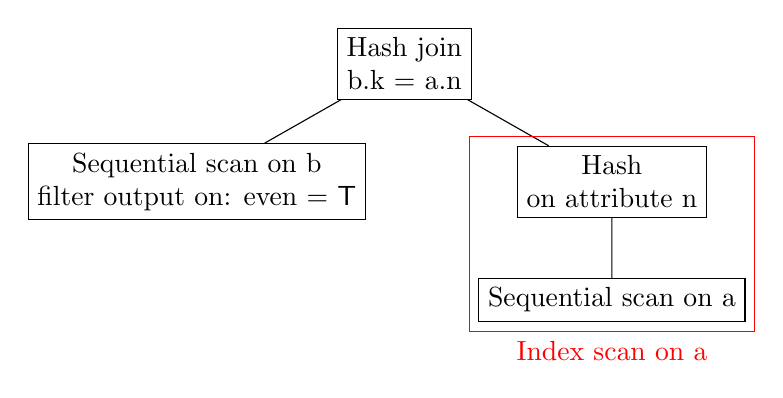
\begin{tikzpicture}[sibling distance=15em,
  every node/.style = {shape=rectangle,
    draw, align=center}]]
  \node {Hash join\\ b.k = a.n}
    child { node {Sequential scan on b\\ filter output on: even = \textsf{T}} }
    child { node (a) {Hash\\ on attribute n}
      child { node (b) {Sequential scan on a} } };

    \node[fit=(a) (b), rectangle, draw=red, label=below:{\color{red} Index scan on a}] {};
\end{tikzpicture}

  \end{minipage}
  \caption{The query execution plan associated to figure~\ref{ex_relalg}}
  \label{postgres_QEP}
\end{figure}

\subsubsection{Query execution}
\label{query_execution}
Given a relational algebra term, the DBMS elaborates a concrete \emph{query execution plan} (QEP).
A QEP takes the form of a binary tree whose nodes are \emph{physical, low-level algorithms} that effectively treat and output the data in memory.
A same relational algebra term is implemented by several QEPs, with different expected running times.
These running times vary in particular with the size of tables: a small relation will be more efficiently treated as is,
while a large relation may benefit from building dedicated indexing structures.
The RDBMS tries to choose the fastest QEP to execute a query.
A detailed exposition of PostgreSQL QEPs can be found in~\cite{postgresql_manual}, section 14.1: \emph{Using EXPLAIN}.
The QEP generated by PostgreSQL for the query presented in figure~\ref{ex_relalg} is detailed in figure~\ref{postgres_QEP}.

Notice how the join comes last in the QEP while it came first in the relational algebra term.
Indeed, multiple abstract terms (respectively QEPs) are available to describe (resp. execute) a same query.
The rewrite rules that transform relational algebra terms while preserving their interpretation are called \emph{algebraic equivalences}.
They have been proven correct by DataCert and are briefly described in Benzaken et al.~\cite{CFRDM}.

The structure on which a QEP is built is known as the \emph{physical algebra}.
Low-level algorithms are operators of that algebra, while terms are either \emph{iterators} or \emph{indices}.

\paragraph{Iterators.}

A tuple iterator is an abstract list-like data container on which it is possible to perform the following operations:
\begin{itemize}[topsep=0pt, noitemsep]
\item the \emph{init} operation allocates whatever data structure in memory is necessary for iterating data: it is a required preliminary operation;
\item the \emph{next} operation produces a tuple (or tuple address) and alters the internal data structures of the iterator to reflect it;
\item the \emph{close} operation terminates the iterator's operation, by e.g. deallocating memory.
\end{itemize}

The QEP ultimately generates an iterator over all the tuples that were selected by the original request.
The abstract representation of an iterator (called \coqe{Cursor}...) from~\cite{CFSEE} is partially reproduced in figure~\ref{iterator_model}.

\subparagraph{Cursors.} The concept of iterator is inseparable from the notion of \emph{cursor}. A cursor serves to remember previous operation of the iterator, and points to whatever corresponds to the current state of the iteration. Most iterators will use an adequate cursor internally. We have defined cursors for various data structures, namely association lists, hashtables and B+trees (see section~\ref{btree_section}).

\begin{figure}
  \begin{minipage}{0.45\textwidth}
  \begin{coq}
Record Cursor (elt : Type) : Type := {
  cursor: Type;
  next: cursor -> result elt * cursor;
  has_next: cursor -> Prop;
  \end{coq}\end{minipage}\hfill
  \begin{minipage}{0.45\textwidth}
  \begin{coq}
  reset: cursor -> cursor;
  collection: cursor -> list elt;
  visited: cursor -> list elt;
  coherent: cursor -> Prop; [...] }
  \end{coq}\end{minipage}
  \caption{DataCert iterators, without axioms}
  \label{iterator_model}
\end{figure}

\paragraph{Indices.}

Database indices are efficient implementations of the \emph{finite map} interface, that can quickly tell the DBMS where a tuple is situated in memory.

Finite maps represent finite functional relations between keys and values, that is, relations that can be represented by a (partial) function,
where keys map to a unique value.
Let $\mathcal{M}(K, V)$ be the abstract type of finite maps storing keys of type $K$ and values of type $V$.
The minimal interface has two operations $\lookup\!: K \rightarrow \mathcal{M}(K,V) \rightarrow \mathsf{option}\ V$
and $\Insert\!: K \rightarrow V \rightarrow \mathcal{M}(K,V) \rightarrow \mathcal{M}(K,V)$, where $\mathsf{option}$ is the usual option functor.
It also has an \emph{empty} map $m_\emptyset: \mathcal{M}(K,V)$.
These operations must satisfy the following axioms:
\begin{equation} \begin{array}{rcl}
  \forall k, \quad \lookup k\ m_\emptyset & = & \mathsf{None} \\[.2cm]
\forall k\ \forall k'\ \forall m, \quad
\lookup k'\ (\Insert k\ v\ m) & = & \left\{
\begin{array}{cl}
  \some v & \mathrm{if}\quad k = k'\\
  \lookup k'\ m  & \mathrm{otherwise.}
\end{array} \right. 
\end{array} \label{map_axioms}\end{equation}

\textsf{lookup} can be used to define an implementation-agnostic equivalence relation $\equiv$ on maps, stating that two maps hold exactly the same mappings:
\[ \forall m\ \forall m',\quad m \equiv m' \qquad \overset{\mathrm{def}}{\Leftrightarrow} \qquad \forall k,\quad \lookup k\ m = \lookup k\ m' \]
which then yields the properties:
\[\begin{array}{rrcl}
& \Insert k\ v'\ (\Insert k\ v\ m) & \equiv & \Insert k\ v'\ m \\
\text{and if } k \neq k', & \Insert k'\ v'\ (\Insert k\ v\ m) & \equiv & \Insert k\ v\ (\Insert k'\ v'\ m)\ .
\end{array}\]

\subparagraph{Concatenated indices.}
Using C pointers, it is possible to accomodate any type for values by refering to their addresses in memory.
However, known concrete implementations of indices usually handle atomic key types only, like integers (B+trees) or strings (tries).
But what if we want to index data on a product type $K_1 \times K_2$?

The solution consists in implementing $\mathcal{M}(K_1 \times K_2, V)$ as $\mathcal{M}(K_1, \mathcal{M}(K_2, V))$.
Given $(k_1, k_2): K_1 \times K_2$ and $m: \mathcal{M}(K_1, \mathcal{M}(K_2, V)$, we implement the interface for $\mathcal{M}(K_1 \times K_2, V)$ by posing
\begin{align*}
\tilde{m}_\emptyset & := m_\emptyset \\
\mathsf{lookup\_or\_empty}\ k\ m & := \mathrm{if}\ \lookup k\ m = \mathsf{Some}\ v \ \mathrm{then}\ v \ \mathrm{else}\ m_\emptyset\\
\widetilde{\lookup} (k_1, k_2)\ m & := \lookup k_2\ (\mathsf{lookup\_or\_empty}\ k_1\ m)\\
\widetilde{\Insert} (k_1, k_2)\ v\ m & := \Insert k_1\ (\Insert k_2\ v\ (\mathsf{lookup\_or\_empty}\ k_1\ m)\ m\ .
\end{align*}

The proof that these definitions verify the axioms~\eqref{map_axioms} is easy and, due to space constraints, left to the reader.
\emph{Concatenated indices} refer to such maps where the key type is composite;
they are used to index tuples based on their projection on a list of attributes called a \emph{subschema}.

\subparagraph{Primary and secondary indices.}
\emph{Entity integrity} is a database concept meaning that all the tuples in a database must be
uniquely identifiable and capable of being located~\cite{DGS}.
To maintain it, RDBMSs require relations to have a \emph{primary key},
i.e. a subschema of the relation on which each tuple's projection is unique.
While it is possible to define as primary key the whole schema if no two tuples are identical,
that would be less performant than finding an adequate and minimal primary key.

RDBMSs systematically build an index on the primary key of a relation: it is called the \emph{primary index} and defines the relation's content.
That primary index is usually a B+tree when the primary key is composed of a single integer field, because they allow ordered iteration (see section~\ref{btree_section}).

RDBMSs can also build \emph{secondary indices} indexing tuples on other attributes.
Since tuples do not necessarily have unique projections on these attributes,
a secondary index implements a finite map whose values are lists or iterators,
or equivalently a kind of finite map interface with duplicates.

\paragraph{Iterator- and index-generating algorithms}
Here is a description of the database algorithms that I implemented.
\begin{itemize}[itemsep=1pt, topsep=0pt]
\item The \emph{sequential scan} outputs an iterator over \emph{all} the tuples stored in a relation $R$.
It relies on the primary index of $R$ and doesn't take any other input, thus lies at a leaf of the QEP.
\item The \emph{index scan} indexes tuples in a relation based on their projection on a given sub-schema.
Its pseudo-code is in algorithm~\ref{index_scan_algo}.
The $\Insert^\text{list}$ function implements the insertion of an element $v: V$ at key $k: K$ in a ``finite map with duplicates'' of type $\mathcal{M}(K,\ \mathsf{list}\ V)$:
if no mapping is found at key $k$, a singleton list $[v]$ is inserted. Otherwise, the current list $l_k$ of values corresponding to key $k$ is retrieved, $v$ added to it, and the new list $v :: l_k$ is inserted back.

\begin{algorithm}
 \KwData{A relation $R$ and a subschema $(A_i)_{i=1}^n$ of $R$.}
 \KwResult{A secondary index based on that subschema.}
 $m: \mathcal{M}(D_1 \times \dots \times D_n,\ \mathsf{list}\ P) := m_\emptyset$\\
 \qquad where $\forall i$, $D_i$ is the domain of $A_i$ and $P$ is the type of heap pointers\;
 $\mathsf{it}$ := the sequential scan iterator on $R$\;
 $\mathsf{it.init()}$\;
 \While{$\mathsf{it}$ is not empty}{
  (tuple) $t$ := $\mathsf{it.next()}$\;
  $t_\text{proj} := \pi_{(A_i)_i}(t)$\;
  $m := \Insert^\text{list} t_\text{proj}\ \&t\ m$;
 } $\mathsf{it.close()}$\;
 \KwRet{$m$}
 \caption{The index scan algorithm}\label{index_scan_algo}
\end{algorithm}

\item The \emph{index join} is a fast implementation of the $\bowtie$ abstract operator.
  When computing $R \bowtie R'$ and by analogy with the nested-loop algorithm, $R$ will be called the \emph{outer relation}
  and $R'$ the \emph{inner relation}.
  The index join uses a secondary index to lookup all tuples from the inner relation that can be joined with a given tuple from the outer relation.
  Its interface is in algorithm~\ref{index_join_algo} and its implementation in C is partially detailed in section~\ref{implementation}.
  The interested reader can find detailed complexity analysis as well as descriptions of other efficient algorithms for joining relations in Mishra and Eich~\cite{JPRD}.
  \begin{algorithm}
    \KwData{An iterator $\mathsf{it}$ on relation $R^\text{out}$ with schema $(A_i)_i$,\\
      the schema $(B_j)_j$ of $R^\text{in}$,\\
      a list of pairs of foreign keys $(A_{i_k}, B_{j_k})_{k = 1}^m$,\\
      a secondary index $m: \mathcal{M}(D_1 \times \cdots \times D_m,\ \mathsf{list}\ P)$ on the subschema $(B_{j_k})_k$ of $R^\text{in}$}
    \KwResult{An iterator on $R^\text{out} \bowtie_{\bigwedge_k (A_{i_k} = B_{j_k})} R^\text{in}$}
    \caption{The classic index (equi)join algorithm: interface}
    \label{index_join_algo}
  \end{algorithm}
\end{itemize}
\section{Implementation of some low-level algorithms in C}
\label{implementation}
When I started my internship, DeepSpecDB already had some libraries implementing the main data structures used to index tuples' addresses in memory:
B+trees~\cite{Tosin}~\cite{Aurele}, hashtables, association lists.
I developed database code that would use these libraries and implement the sequential scan, index scan and index join algorithms. 

\subsection{Object-oriented programming in C}

Assume that in a query execution plan, an algorithm $A$ takes input from iterators $\textit{it}_1$ and $\textit{it}_2$.
The implementation of $A$ only needs to have access to the \emph{init}, \emph{next} and \emph{close} operations of $\textit{it}_1$ and $\textit{it}_2$.
Moreover, we don't want the implementation of $A$ to depend on what algorithm yields $\textit{it}_1$ or $\textit{it}_2$.
This modularity is achieved through an \emph{object-oriented} approach.

Object-oriented (OO) programming in C needs explicit method closures, as the language doesn't have built-in OO patterns.
A C object can be implemented as a structure with a pointer to a \emph{method table}, that stores function pointers to methods,
and a pointer to an \emph{environment} that stores private data.
A \emph{class interface} or \emph{abstract class} or \emph{signature} specifies the names of the methods and the types they must have.
An object \emph{class} describes a set of objects that have common methods with the same implementation.
A class can implement an interface, in which case the interface's methods must be a subset of the class's methods.
In our case, the abstract class or interface is ``the iterators'' and the classes are the physical iterator-generating algorithms.

The C type of environments can vary between different classes implementing the same interface,
in order to account for different method implementation.
That feature is achieved through pointer casts. The generic environment pointer has type \ce{void*}.

For example, instances of the sequential scan iterator class have an environment composed of a B+tree primary index pointing to a relation, and a cursor on that B+tree.
The cursor is initialized to the first position by \emph{init}, and moved to the next record by \emph{next}.
However, the methods and environment of the index join are completely different (see next section).

\noindent\begin{minipage}{.45\textwidth}
  \begin{lstlisting}[language=C, basicstyle=\small]
    struct methods {
      void (*init) (void* env);
      const void* (*next) (void* env);
      void (*close) (void* env);
    };
\end{lstlisting}\end{minipage}\hfill
\begin{minipage}{.45\textwidth}
  \begin{lstlisting}[language=C, basicstyle=\small]
    typedef struct iterator_t {
      struct methods *mtable;
      void* env;
    } *iterator;
  \end{lstlisting}
\end{minipage}\\

It is particularily unsafe to call methods directly, as there is no restriction on what the environment pointer actually points to.
I therefore also defined convenient wrappers around an iterator's methods, like this \ce{get_next} function, which guarantees that
an iterator's \ce{next} method is always called with the iterator's environment:
\begin{lstlisting}[language=C, basicstyle=\small]
  const void* get_next(iterator it) { return it->mtable->next(it->env); };
\end{lstlisting}

\subsection{The index join: implementation}\label{actual_implementation}
\def\inlinec{\lstinline[language=C, basicstyle=\normalsize, columns=fixed]}

This section details the implementation of the \ce{next} method of the index join iterator.
That code implements the relational algebraic equijoin, modified to delete duplicate columns, as explained in section~\ref{relmodel}.

{\lstset{language=C, basicstyle=\footnotesize, numbers=left, mathescape}
\begin{lstlisting}
const void* index_join_next(void* env) {
  struct index_join_env* e = (struct index_join_env*) env;$\label{env_cast}$
\end{lstlisting}
\lstset{firstnumber=last}

The defined function has the expected prototype for a \inlinec{next} method.
Line~\ref{env_cast} casts the generic environment pointer into the index join's own environment pointer type.
The index join environment holds essential data like the schema of both relations, the outer iterator,
and the index on the inner relation.

\begin{lstlisting}
  while((e->current_inner == NULL || fifo_empty(e->current_inner))
        && (e->current_outer = get_next(e->outer)) ) {
    Key proj = get_projection(e->outer_attrs, e->current_outer, e->outer_join_attrs);
    e->current_inner = (fifo*) index_lookup(e->ind_on_inner_sch, e->ind_on_inner, proj);
  };
\end{lstlisting}

If the inner relation has no more tuple that matches the projection on join attributes of the current outer tuple,
we query a new outer tuple from the outer iterator using \inlinec{get_next}.
In that case, we also retrieve the list (\inlinec{fifo}) of inner tuples from the inner index
that can be joined with the current outer tuple.

\begin{lstlisting}
  if(!e->current_outer) return NULL;$\label{after_if}$
\end{lstlisting}

That \lstinline[columns = fixed]{if} statement is triggered when the outer tuple iterator is now empty: the index join iterator is now also empty,
thus the \emph{next} method returns the null pointer.

Past line~\ref{after_if}, we now have an outer tuple \inlinec{e->current_outer} that has to be joined with \emph{all} the inner tuples
that are stored in the inner tuple list \inlinec{e->current_inner}.

\begin{lstlisting}[language=C]
  size_t outer_t_length = attribute_list_length(e->outer_attrs);$\label{all1}$
  size_t inner_t_length = attribute_list_length(e->inner_attrs);$\label{all2}$
  size_t join_length = attribute_list_length(e->inner_join_attrs);$\label{all3}$
\end{lstlisting}

Lines~\ref{all1}, \ref{all2} and \ref{all3} calculate the respective number of attributes in
the outer tuples,
the inner tuples, and
the list of inner attributes that are going to be identified with the attributes from \inlinec{outer_join_attrs} by the join algorithm.
In the actual implementation, these numbers are calculated only once by \emph{init}.

Crucial to understanding the rest of the code are the following statements:
\begin{enumerate}[noitemsep, topsep=0pt, label=(\alph*)]
\item a single tuple is stored contiguously in memory, and
\item independently of its domain, a field in a tuple occupies exactly \inlinec{sizeof(void*)} bytes of memory, which is 8 on a 64-bits machine.
This does \emph{not} depend on whether the domain of that field is integer or string.
Integer entries in our system are \inlinec{unsigned long} and thus occupy 8 bytes and a string field is a pointer to the string characters, which is also 8 bytes.
Note that unfortunately, these facts are not specified in the C standard, thus the code may not be portable.
\end{enumerate}

\begin{lstlisting}
  void* new_t = malloc(sizeof(void*)*(outer_t_length + inner_t_length - join_length + 1));
  memcpy(new_t, e->current_outer, sizeof(void*) * outer_t_length);
\end{lstlisting}

We allocate the memory space for the new joined tuple, calculating its size (in multiples of 8 bytes) using the length of the various attribute lists.
Data from the outer tuple is entirely copied at the beginning of that new location.

\begin{lstlisting}
  const void* inner_t = fifo_get(e->current_inner)->data;
  attribute_list l = e->inner_attrs;
\end{lstlisting}

We retrieve the next inner tuple in the list and create an alias for the list of the inner schema.

\begin{lstlisting}
  size_t n = 0;
  for(; l != NULL; l=l->next) {
\end{lstlisting}

This loop will copy in the new joined tuple all fields in \inlinec{inner_t} that are not already present.

\begin{lstlisting}
    size_t inner_t_ofs = get_offset(e->inner_attrs, l->id, l->domain);
\end{lstlisting}

\inlinec{get_offset(attrs, attr_name, attr_domain)} returns the integer index of \inlinec{attr_name} in the attribute list \inlinec{attrs}, or a negative number if \inlinec{attr_name} is not found.
The \inlinec{attr_domain} parameter allows to fail if \inlinec{attr_name} exists in attrs, but with a different domain.
An optimized version of the code would calculate the offsets only once at initialisation.

\begin{lstlisting}
    if(get_offset(e->inner_join_attrs, l->id, l->domain) < 0) {
      memcpy((void*) (((size_t*) new_t) + outer_t_length + n),
          (void*) ((size_t*) inner_t + inner_t_ofs), sizeof(size_t));
      n++;
    };
  }
  return new_t;
};
\end{lstlisting}
}

Finally, the index join is packaged into the iterator structure with its other methods whose details have been omitted here:

\begin{lstlisting}[language=C, basicstyle=\footnotesize, mathescape]
struct methods index_join_iterator_mtable =
     { &index_join_init, &index_join_next, &index_join_close };

iterator index_join($[...]$) {
  $[...]$
  struct index_join_env *env = malloc(sizeof(struct index_join_env)); if(!env) exit(1);
  $[... \text{initialize the environment structure} ...]$
  iterator it = malloc(sizeof(struct iterator_t)); if(!it) exit(1);
  it->mtable = &index_join_iterator_mtable;
  it->env = (void*) env;
  return it;
}
\end{lstlisting}

\subsection{Verification: perspective}

Verification of object-oriented C code using Verifiable C is described by Appel et al.~\cite{PLCC}, chapter 29: \emph{Dependently typed C programs}.
The method that is presented will involve defining a generic Coq record type for the \inlinec{iterator} abstract class that contains various definitions about the separation logic representation of iterators
and proof of statements about these definitions.
That Coq record defines what should be common to all implementations of iterators with respect to Verifiable C logic.

I have attempted at verifying that code, however I realized that it was too early to do so since the building blocks
like indices were not done yet.
Also, given that specifications are usually subtly modified as the proof is carried out,
I will not reproduce here my attempts as they have not yet be proven to be fully correct.
No Verifiable C verification has ever been attempted on such a large object-oriented code base.

\section{A verified hashtable program}
\label{hashtable}
I achieved the verification of an implementation of \emph{hashtables with external chaining}, that was used in our implementation of concatenated indices. The Verifiable C tutorial~\cite{VCT} guides students through the verification of a hashtable implementing a string multiset algebraic datatype by mapping string keys to their multiplicity in the multiset. The separation logic proof technique that is used is called \emph{Magic wand as frame} and is the object of a recent paper~\cite{MWAF} co-authored by my supervisor.

I will explain in this section how the Verifiable C verification of DeepSpecDB's integer hashtables led me to instantiate the magic-wand-as-frame technique in an interesting way.

\subsection{Purpose and C code}

As explained in section~\ref{query_execution}, we need to be able to build various kinds of indices for the join algorithm. Each of our attribute domains - strings or integers for now - has its own implementation of a key-pointer store: string association lists and integer hashtables, respectively. A concatenated index is implemented as an index pointing to other indices.

The hashtable data structure consist of an array of pointers to linked lists, called buckets. The bucket at array position $i$ contains any entry whose integer key $k$ verifies $k\ \mathrm{mod}\ N = i$, where $N$ stands for the total number of buckets in the array. \emph{External chaining} means that the hashtable handles collisions of hashes of different keys by growing the linked list buckets.
We use a large and prime $N$, namely 65599, to distribute entries evenly on average and guarantee fast lookups.

The insertion operation has a main procedure \ce{inthash_insert} and an auxiliary function \break\ce{inthash_insert_list} that are both reproduced in figure~\ref{inthash_insert}.

\begin{figure}
\begin{minipage}{0.5\textwidth}
\begin{lstlisting}[language=C,basicstyle=\small]
struct icell {
  size_t key;
  void *value;
  struct icell *next;
};
\end{lstlisting}
\end{minipage}\hfill
\begin{minipage}{0.5\textwidth}
\begin{lstlisting}[language=C, basicstyle=\small]
struct inthash {
  struct icell *buckets[N];
};
\end{lstlisting}
\end{minipage}
\begin{lstlisting}[language=C,basicstyle=\small, numbers=left, escapechar=|]
struct icell *inthash_insert_list (struct icell **r0, size_t key) {
  struct icell *p, **r;
  for(r=r0; ; r=&p->next) { |\label{begin_loop}|
    p = *r;
    if (!p) {
      p = new_icell(key,NULL,NULL);
      *r = p;
      return p;
    }
    if (p->key==key) {
      return p;
    }
  } |\label{end_loop}|
}

void* inthash_insert (inthash_t p, size_t key, void *value) {
  struct icell *q;
  void *old;
  q=inthash_insert_list (& p->buckets[key%N], key);
  old=q->value;
  q->value=value;
  return old;
}
\end{lstlisting}
\caption{Hashtable definition and insertion}
\label{inthash_insert}
\end{figure}

\begin{figure}
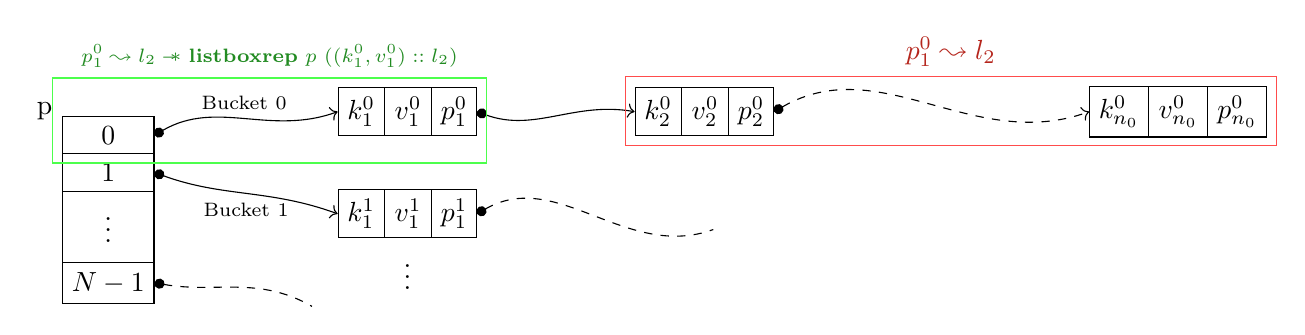
\begin{tikzpicture}

\node[rectangle split, draw, rectangle split parts = 4, label={120:p}] (bs) {0 \nodepart{two} 1 \nodepart{three} \strut $\vdots$ \nodepart{four} $N - 1$};

\node[rectangle split, rectangle split part align=base, rectangle split horizontal, draw, rectangle split parts = 3, above right = 1mm and 3cm of bs.one] (b11) {$k^0_1$ \nodepart{two} $v^0_1$ \nodepart{three} $p^0_1$};

\draw[{Circle}->] (bs.one east) to [out=30,in=200] node[above]{\scriptsize{Bucket 0}} (b11.one west);

\node[rectangle split, rectangle split part align=base, rectangle split horizontal, draw, rectangle split parts = 3, right = 2cm of b11.east] (b12) {$k^0_2$ \nodepart{two} $v^0_2$ \nodepart{three} $p^0_2$};

\draw[{Circle}->] (b11.east) to [out=-20,in=170] (b12.one west);

\node[rectangle split, rectangle split part align=base, rectangle split horizontal, draw, rectangle split parts = 3, right = 4cm of b12.east] (b1n) {$k^0_{n_0}$ \nodepart{two} $v^0_{n_0}$ \nodepart{three} $p^0_{n_0}$};

\draw[{Circle}->, dashed] (b12.east) to [out=30,in=200] (b1n.one west);

\node[rectangle split, rectangle split part align=base, rectangle split horizontal, draw, rectangle split parts = 3, below right = 1mm and 3cm of bs.two, label={-90:$\vdots$}] (b21) {$k^1_1$ \nodepart{two} $v^1_1$ \nodepart{three} $p^1_1$};

\draw[{Circle}->] (bs.two east) to [out=-20,in=160] node[below]{\scriptsize{Bucket 1}} (b21.one west);

\draw[{Circle}-, dashed] (b21.east) to [out=30,in=200] +(3, -.2);

\draw[{Circle}-, dashed] (bs.four east) to [out=-10,in=150] +(2, -.3);

\node[rectangle, fit=(b12.south west) (b1n.north east), draw = red!70, label={\color{BrickRed} $p^0_1 \leadsto l_2$}] {};

\node[rectangle, fit=(bs.one split west) (b11.north east), draw=green!70,
  label={\color{ForestGreen} \scriptsize{$p^0_1 \leadsto l_2 \wand \mathbf{listboxrep}\ p\ ((k^0_1, v^0_1) :: l_2)$}}] {};

\end{tikzpicture}
\caption{Hashtable illustration and separation logic predicates, where $l_2 := [(k^0_2, v^0_2), \dots, (k^0_{n_0}, v^0_{n_0})]$ and $p$ is the address of the first bucket pointer.}
\label{hashtable_drawing}
\end{figure}

The \ce{inthash_insert_list} function returns a pointer to the adequate cell in a bucket, by creating a new cell if needed.
The pointed cell has to be updated with the new value by the \ce{inthash_insert} function, which itself returns the old value.

\subsection{Separation logic representation}

Notice that the \ce{inthash_insert_list} function can modify the pointer in the bucket array, in the case the bucket is empty, hence the use of a pointer to a pointer in the arguments of the function. The paper and the Verifiable C tutorial describe such a situation using a \textbf{listboxrep} predicate, along with the standard separation logic representation predicate for linked lists:
\[ \begin{array}{ll}
  p \leadsto \mathrm{nil} & :=\ p = \mathrm{null}\\
  p \leadsto (k, v)::\mathit{tl} & :=\ p.\mathsf{key} \mapsto k * p.\mathsf{value} \mapsto v * \exists q, p.\mathsf{next} \mapsto q * q \leadsto \mathit{tl}\\[.3cm]
  \mathbf{listboxrep}\ l\ p & := \exists q, p \mapsto q * q \leadsto l \end{array} \]

The notations are as follows:
\begin{itemize}[noitemsep, topsep=0pt]
  \item $*$ is the separating conjunction: a heap $m$ satisfying $A * B$ (written $m \models A * B$) can be split into two disjoint parts $m_1$ and $m_2$ such that $m_1 \models A$ and $m_2 \models B$;
  \item $p \mapsto v$ means that value $v$ is stored at memory address $p$ on the heap; 
  \item $\mathrm{nil}$ is the empty list and $::$ is the constructor of functional lists - in this case, association lists or lists of pairs;
  \item finally, $\mathrm{null}$ is the null pointer.
\end{itemize}

The separating implication will be denoted $A \wand B$. By definition, $m \models A \wand B$ if and only iff for all $m'$ disjoint from $m$ such that $m' \models A$, we have $m \oplus m' \models B$, where $\oplus$ is heap disjoint union. Intuitively, $A \wand B$ describes a heap $A$ where a part $B$ is missing. 

The magic-wand-as-frame paper advocates the use of that separating implication, or \emph{magic wand}, to describe partial data structures that appear on the heap when a recursive data structure (e.g. binary tree, linked list) is traversed.  The magic wand then allows for elegant loop invariants that \emph{do not} require additional inductive predicates for partial structures to be defined (e.g. list segments or partial trees). The paper shows that this technique can be used when the traversal doesn't modify the heap (e.g. for lookups) but also and more interestingly \emph{when it does}, like here. In the latter case, the wand conjunct has to use a universal quantifier over the remaining sub-structure, to be modified by the traversal. More details are given below.

In the body of \ce{inthash_insert_list} comes a loop (lines~\ref{begin_loop} to~\ref{end_loop}) in which the \emph{pointer value} stored at address \ce{r} goes through the bucket until reaching the end of the linked list or the current mapping for key $k$. With respect to the magic-wand-as-frame technique, I used the following loop invariant:

\[ \begin{array}{rl}
  \exists (l_1, l_2),\ l = l_1l_2\ \wedge\ \llbracket \mathtt{r} \rrbracket = r\ \wedge\ \llbracket \mathtt{r_0} \rrbracket = r_0\ \wedge\ \llbracket \mathtt{k} \rrbracket = k\ *\
   \mathbf{listboxrep}\ r\ l_2\ * & \\
   \forall l_2',\ \mathbf{listboxrep}\ r\ l_2'\ \wand\ \mathbf{listboxrep}\ r_0\ (l_1l_2') & \end{array}\]

The concatenation of two lists $l_1$ and $l_2$ is written $l_1l_2$ above. The universal quantification on the sublist whose starting address is stored at $r$ before the wand means that using that loop invariant, it is possible to alter that list when needed. In the case of \ce{inthash_insert_list}, that happens when a new cell has to be added at the end, because the key being searched wasn't found. In that case, the new cell will be given the \ce{NULL} mapping. That value will be modified by the \ce{inthash_insert} function.

When specifying \ce{inthash_insert_list}, it is necessary to include the fact that the returned value is pointing to the list cell that needs to be modified by \ce{inthash_insert}. I thus came up with the following specification:
\[ \begin{array}{cl}
   \mathrm{(precondition)} & \{ \llbracket \mathtt{p} \rrbracket = p \wedge \llbracket \mathtt{k} \rrbracket = k \wedge \mathbf{listboxrep}\ l\ p \}\\
  \mathrm{(statement)} & \qquad p_\mathrm{ret} = \mathtt{inthash\_insert\_list(p, k)}\\
  \mathrm{(postcondition)} & \{ \exists (r, v_0, \mathit{tl}),\ r \mapsto p_\mathrm{ret} * p_\mathrm{ret} \leadsto (k, v_0)::\mathit{tl}\ *\\
  & \qquad \qquad \forall v,\ r \mapsto p_\mathrm{ret} * p_\mathrm{ret} \leadsto (k, v)::tl \wand \mathbf{listboxrep}\ (\mathbf{add}\ k\ v\ l)\ p\}
\end{array} \]

Here, $\mathbf{add}$ is the insertion on functional association lists.
To have a sufficiently strong postcondition, it is \emph{not possible} to use the \textbf{listboxrep} predicate for the two first conjuncts and before the wand in the postcondition.
If we do, because of the existential quantification in \textbf{listboxrep} on the value stored at $r$, we lose the information that the returned value $p_\mathrm{ret}$ points to a sublist whose head key is the inserted key.
That's why, contrary to the paper's examples, I had to unfold the definition of \textbf{listboxrep}.

Notice how adequate and specific to the problem that specification is. Once \ce{inthash_insert_list} is proven to conform to that specification, the proof of \ce{inthash_insert} - with a natural specification matching the new hashtable in the heap with the same hashtable where key $k$ now maps to value $v$ - goes very smoothly, because most of the work is done in that auxiliary proof.

Finally, the C code could have been modified in the following way: pass the new value to\linebreak\ce{inthash_insert_list}, and make it perform the update and return the old value. In that case, we wouldn't have had to give a magic-wand postcondition for \ce{inthash_insert_list}, which may have been a little simpler. However, it is interesting to see that the magic-wand-as-frame technique can be adapted to various situations like this piece of C code.

\section{A verified B+tree functional implementation}
\label{btree_section}
B+trees are a specific kind of multiway search trees that store ordered mappings of a key to an associated value. B+trees are derived from B-trees, which were originally described by Bayer and McCreight~\cite{OMLOI}. B+trees have been designed to handle massive amounts of data while allowing for the shortest lookup time. Such trees are typically very wide and shallow, so that the number of nodes fetched from cold areas of cache or main memory on a path from the root to a leaf is small. The number of children of a node is also chosen so as to minimize cache misses, that is, so that one node of a B+tree is the same size as the block size of one layer of the memory hierarchy (disk or cache).

This section describes the B+tree data structures and its invariants, then exposes some challenges I faced during formalization in Coq.

\subsection{Presentation of B+trees}
\label{btree_maths}
Informally, B+tree nodes have the following structure. A \emph{leaf node} will contain a number of \emph{entries} which are key-value pairs and solely constitute the information contained in the abstract key-value store.
An \emph{internal node} contains a \emph{zero} (or \emph{leftmost}) \emph{pointer} and a list of key-child pointer pairs - also called entries. The entry keys guide the lookup operation towards the right mapping in the appropriate leaf. The lookup top-to-bottom traversal is similar to that of any binary search tree - except that the number of children is greater. Contrary to B-trees, B+tree internal nodes do not carry any mapping information: their only purpose is to make lookups fast using intermediate keys. 

Formally, the inductive definition of the base type of the B+trees is the following:
\[ t \quad = \quad T(t_0, (k_i, t_i)_{i = 1}^{n_t})\quad | \quad L((k_i, v_i)_{i = 1}^{n_t}) \]
where $t, t_0, t_1, \dots, t_{n_t}$ are trees, the $k_i$'s are keys, the $v_i$'s are values, a pair $(k, x)$ where $k$ is a key and $x$ is either a tree or a value is called an \emph{entry}, and the number $n_t$ of entries is tree-dependent.
The words \emph{tree} and \emph{node} will be used interchangeably in the rest of the explanations. The constructor $T$ refers to internal nodes, while $L$ refers to leaves.

Along with that definition, we will use the usual notions of \emph{child}, \emph{tree path} and \emph{path length}.
An internal node $T(t_0, (k_i, t_i)_{i = 1}^{n_t})$ has $n_t + 1$ children, which are trees $t_0, t_1, \dots, t_{n_t}$. That is, the leftmost pointer is a child, and so are the trees in the entries.
Leaf nodes have no child. If $t_\text{child}$ is a child of $t_\text{parent}$, we write $\mathsf{child}\ t_\text{child}\ t_\text{parent}$.
A path will be an ordered collection of distinct nodes $(t_0, t_1, \dots, t_d)$ such that $\forall i \in \{0, \dots, d - 1\},$ $t_{i + 1}$ is a child of $t_i$.
Such a path is said to have length $d$, which is the number of edges it is composed of.

A node $t_\text{child}$ is said to be a \emph{subnode} of another node $t_\text{parent}$ if there is a path from $t_\text{parent}$ to $t_\text{child}$.
That defines a predicate and we write $\mathsf{subnode}\ t_\text{child}\ t_\text{parent}$.
The $\mathsf{subnode}$ relation is the reflexive transitive closure of the $\mathsf{child}$ relation.

Given such a multiway tree $t$ and a positive integer $m \in \mathbb{N}_{>0}$, we say that $t$ is a B+tree of order~$m$ if it satisfies the following invariants.
\begin{enumerate}
  \itemsep0em
  \item $t$ is \emph{balanced} in the sense that \emph{all paths from t to one of its leaves have the same length}. That length is called the \emph{depth} of the B+tree.

    That property guarantees that looking up any key in the tree will have the same time complexity.
    It is an even stricter balancing invariant than the one of \emph{AVL trees}, which are binary search trees allowing pairs of subtrees to have a height difference of 1.
    This invariant is concomitant to the way an insertion is performed:
    as we will see, during B$\pm$tree insertion, a new node is always a sibling of another preexisting node, or a new root; in other words, B$\pm$trees grow in height at the root, not the leaves.
    That behavior is inherited from 2-3 trees, of which B-trees are a generalization.
  \item $t$ is \emph{well-sized}, that is $t$ has at most $2 * m$ entries and any strict subnode of $t$ has between $m$ and $2 * m$ entries.
    If $t$ is not a leaf, then $t$ must also have at least 1 entry: no internal node has an empty list of entries.

    That invariant guarantees that the complete B$\pm$tree will have a number of nodes that is not too high compared to the number of mappings it contains. The interest of that invariant is to rule out nearly-empty nodes.
In the early days of databases, all the data was stored on slow discs, and a B+tree node's entries would be stored in a dedicated sector or block.
Having nodes with few entries would increase disk usage as well as the total depth of the tree, which decreases cache locality of the program and makes lookups slower.
    The same reasoning applies today to RAM blocks and/or cache lines.
  \item \label{} $t$ is a \emph{search tree}. That property is crucial not for performance, but for proper operation.

    For a leaf node $L((k_i, v_i)_{i = 1}^{n_t})$, we demand that the list of keys $k_1, \dots, k_{n_t}$ be sorted, with respect to whatever strict total order the type of keys comes equipped with.
    A B+tree doesn't allow duplicate keys, however an implementation allowing them seems feasible.

    For an internal node $t = T(t_0, (k_i, t_i)_{i = 1}^{n_t})$, we require that
    \begin{enumerate}
      \item the list of keys $k_1, \dots, k_{n_t}$ is sorted;
      \item all the children of $t$ are search trees;
      \item all keys $k$ in $t_0$ are such that $k \le k_0$ (remember that, if the tree is well-sized, then $n_t > 0$, so $k_0$ exists);
      \item for any $i \in \{1, \dots, n_t - 1\}$, the keys $k$ in $t_i$ are such that $k_i < k \le k_{i + 1}\ $; and
      \item the keys $k$ in $t_{n_t}$ are such that $k > k_{n_t}$.
    \end{enumerate}

\end{enumerate}

\begin{figure}
\centering
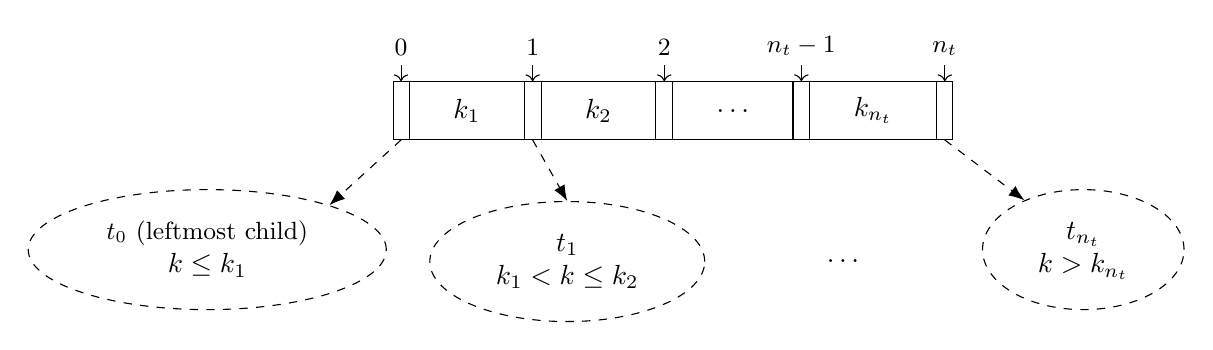
\begin{tikzpicture}
  \node[draw, rectangle split, rectangle split horizontal, rectangle split empty part width=-10, rectangle split parts = 9, inner sep = 2mm] (n)
       {\nodepart{two} $\quad k_1 \quad$ \nodepart{three} \nodepart{four} $\quad k_2 \quad$ \nodepart{five} \nodepart{six} $\quad \dots \quad$ \nodepart{seven} \nodepart{eight} $\quad k_{n_t} \quad$ \nodepart{nine}};

  \node[above=2mm of n.one north] (lm) {\small{0}}
    edge[->] (n.one north);

  \node[above=2mm of n.three north] {\small{1}}
    edge[->] (n.three north);

  \node[above=2mm of n.five north] {\small{2}}
    edge[->] (n.five north);

  \node[above=2mm of n.seven north] {\small{$n_t - 1$}}
    edge[->] (n.seven north);

  \node[above=2mm of n.nine north] {\small{$n_t$}}
    edge[->] (n.nine north);

  \node[ellipse, dashed, draw, below left= 1.2cm of n.one south] (t0) {\begin{tabular}{c} \small{$t_0$ (leftmost child)} \\ $k \le k_1$ \end{tabular} };

  \node[ellipse, dashed, draw, below right= 1cm and -.8cm of n.three south] (t1) {\begin{tabular}{c} $t_1$ \\ $k_1 < k \le k_2$ \end{tabular}};

  \node[below right = 1.4cm and .2cm of n.seven south] {\dots};

  \node[ellipse, dashed, draw, below right= 1.2cm of n.nine south] (tnt) {\begin{tabular}{c} $t_{n_t}$ \\ $k > k_{n_t}$ \end{tabular}};

  \path[-{Latex[width=1.5mm, length=2mm]}, dashed] (n.one south) edge (t0.20);
  \path[-{Latex[width=1.5mm, length=2mm]}, dashed] (n.three south) edge (t1.north);
  \path[-{Latex[width=1.5mm, length=2mm]}, dashed] (n.nine south) edge (tnt.140);

\end{tikzpicture}
\caption{A B+tree internal node. The numbers above indicate child positions used in B+tree cursors.}
\end{figure}

\begin{figure}
\centering
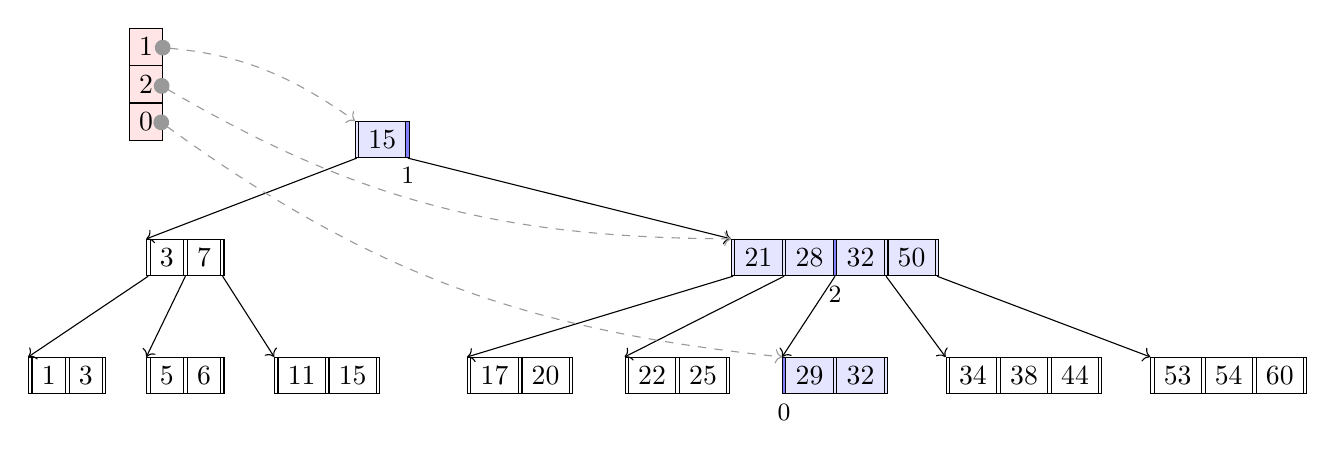
\begin{tikzpicture}[edge from parent/.style={draw=none}]
\tikzstyle{btree_node}=[rectangle split, rectangle split horizontal, rectangle split parts = 5, rectangle split empty part width=-10, draw]

\node [fill=red!10, rectangle split, rectangle split ignore empty parts, draw] at (-3, 0.7) (cursor) {1 \nodepart{two} 2 \nodepart{three} 0};

\node[btree_node, rectangle split part fill = {blue!10, blue!10, blue!50}, rectangle split parts = 3] (root) { \nodepart{two} 15 }
  child[sibling distance = 50mm] {node[btree_node] (d10) {\nodepart{two} 3 \nodepart{four} 7}
    child[sibling distance=15mm] {node[btree_node] (d20) {\nodepart{two} 1 \nodepart{four} 3}}
    child {node[btree_node] (d21) {\nodepart{two} 5 \nodepart{four} 6}}
    child[sibling distance=18mm] {node[btree_node] (d22) {\nodepart{two} 11 \nodepart{four} 15}}    
  } 
  child[sibling distance=115mm] {node[btree_node, rectangle split parts = 9, rectangle split part fill = {blue!10, blue!10, blue!10, blue!10, blue!50, blue!10}] (d11) {\nodepart{two} 21 \nodepart{four} 28 \nodepart{six} 32 \nodepart{eight} 50}
    child[sibling distance=20mm] {node[btree_node] (d23) {\nodepart{two} 17 \nodepart{four} 20}}
    child[sibling distance=20mm] {node[btree_node] (d24) {\nodepart{two} 22 \nodepart{four} 25}}
    child {node[btree_node, rectangle split part fill = {blue!50, blue!10}] (d25) {\nodepart{two} 29 \nodepart{four} 32}}    
    child[sibling distance=24mm] {node[btree_node, rectangle split parts = 7] (d26) {\nodepart{two} 34 \nodepart{four} 38 \nodepart{six} 44}}    
    child[sibling distance=25mm] {node[btree_node, rectangle split parts = 7] (d27) {\nodepart{two} 53 \nodepart{four} 54 \nodepart{six} 60}}    
  };
\path [->] (root.one south) edge (d10.north west);
\path [->] (root.three south) edge (d11.north west);
\path [->] (d10.one south) edge (d20.north west);
\path [->] (d10.three south) edge (d21.north west);
\path [->] (d10.five south) edge (d22.north west);
\path [->] (d11.one south) edge (d23.north west);
\path [->] (d11.three south) edge (d24.north west);
\path [->] (d11.five south) edge (d25.north west);
\path [->] (d11.seven south) edge (d26.north west);
\path [->] (d11.nine south) edge (d27.north west);

%cursor arrows
\path [{Circle[length=2mm]}->, gray!80, bend left = 15, dashed] (cursor.one east)+(-1mm,0) edge (root.north west);
\path [{Circle[length=2mm]}->, gray!80, bend right = 15, dashed] (cursor.two east)+(-1mm,.3mm) edge (d11.north west);
\path [{Circle[length=2mm]}->, gray!80, bend right = 15, dashed] (cursor.three east)+(-1mm,.5mm) edge (d25.north west);

\node[below=0 of root.three south] {\small{1}};
\node[below=0 of d11.five south] {\small{2}};
\node[below=0 of d25.one south] {\small{0}};

\end{tikzpicture}
\caption{A sample B+tree of order 2 and depth 2 showing the ``search tree'' property.
The cursor in light red points to key 29. The nodes on the path designated by the cursor are in light blue.
The numbers in the cursor represent the position of the adequate child or record in the node that is pointed to. The corresponding pointers in the B+tree are highlighted in blue.}
\label{bptree}
\end{figure}

\subsection{Coq model and proofs}

To my knowledge, the only proof assistant formalization of B+trees in the literature is described by Malecha et al.~\cite{TVRDMS}.
Their datatype for B+trees includes a \coqe{nat} height parameter, which allows Coq to check the termination of recursion easily.
They define a tree traversal that is supposed to serve for the implementation of different B+tree operations.
However, they only really use it for insertion, which is the only operation they define along with lookup.
I didn't define or verify the removal operation either, which is expected to be quite lengthy.
However, my formalization is made to match the \emph{cursored} operations we use in our C code.

A B+tree cursor is a path from the root to a leaf record, that is kept in memory by the B+tree C program.
They can be found in the B+tree implementation of SQLite~\cite{DGS}.
They allow speedups on large trees when consecutive lookups and insertions are made \emph{locally} in the tree.
Moreover, they are an alternative to cross-leaf pointers used in most implementations of B+trees~\cite{TVRDMS}~\cite{DSCB} for iterating over all sorted mappings contained in the tree.
A cursor is presented in figure~\ref{bptree}.

Using a cursor, the lookup and insertion operations do not have to traverse the tree from the root.
The leaf where the key is found is reached from the current position of the cursor.
If a sequence of keys is inserted in a sorted or mostly-sorted order, the cursor can provide a noticeable speedup,
because the cursor would move very little, and would trigger fewer cache misses compared to cursorless insertions or lookups, that would need to traverse the whole tree from top to bottom.

My formalization uses a Coq list to describe the entries in a B+tree node, which feels like the most natural way to define multiway search trees.
It takes the form of a Coq functor, and is inspired from the \coqe{FMapAVL} file~\cite{CSTDLAVL} from Coq's standard library,
which implements the finite map interface in \coqe{FMapInterface} using fully verified AVL trees.
However, that part of the standard library is unfortunately deprecated and doesn't seem to be maintained so I chose not to rely on it.

\begin{coq}
Module Type BPlusTreeParams.
  Module InfoTyp.
    Parameter t: Type.
  End InfoTyp.
  Parameter min_fanout: Z.
  Axiom min_fanout_pos: min_fanout > 0.
End BPlusTreeParams.

Module Raw (X: Orders.UsualOrderedTypeFull') (Params: BPlusTreeParams).
  Notation key := X.t.
  Definition entries (elt: Type): Type := list (key * elt).
  
  Inductive node: Type :=
  | leaf (records: entries elt) (info: Info.t): node
  | internal (ptr0: node) (children: entries node) (info: Info.t): node.

  [...]
End Raw.
\end{coq}

Each node stores an \coqe{Info.t} informative value, with no constraint.
The \coqe{min_fanout} parameter corresponds to the $m$ B+tree parameter above.
Keys need to be equipped with a total order.
I have investigated the use of any equivalence relation for equality of keys,
however that was not needed for our purpose and required a lot more work to prove that the non-Leibniz equality was respectful of all other definitions, which is needed for setoid rewriting.
Thus the key type is an instance of \coqe{UsualOrderedType} and not \coqe{OrderedType}.

A \emph{nested inductive type} occurs in the \coqe{children} argument of the \coqe{internal} constructor, as it is a list whose element type contains the inductive type \coqe{node} being defined.
Coq can handle nested inductive types, however I had to convince the termination checker that my inductive definitions on \coqe{node} were terminating, either by structural recursion or using well-founded relations.
An alternative definition uses mutual inductive types to redefine a list of children for \coqe{node}, isomorphic to the Coq type \coqe{list}, but is very impractical given that all definitions and lemmas about lists cannot be reused.

For such nested inductive types, the induction principle automatically defined by Coq is too weak. A proper induction principle can however be proved.
Different choices are possible. I chose the \coqe{Forall} predicate for the induction hypothesis:
\begin{coq}
Lemma node_ind (P: node -> Prop)
  (hleaf: forall records info, P (leaf records info))
  (hinternal: forall ptr0 children info,
      P ptr0 -> Forall P (map snd children) -> P (internal ptr0 children info)):
$\forall$ n, P n.
\end{coq}

Two methods are documented for recursive definitions on such nested inductive types:
\paragraph{Well-founded relations.}
The first method is to use a well-founded relation, or to use a measure and a predefined relation (e.g. less-than on natural numbers).
My take on that was inspired by what is done in the Equations package~\cite{ER}.
Equations has tactics and a command \coqe{Derive Subterm} that try to define automatically a \emph{subterm} relation for recursive inductive types and prove its well-foundedness.
In my case, I defined the following:
\begin{coq}
Inductive child: relation node :=
| child_ptr0: forall ptr0 records info,
    child ptr0 (internal ptr0 records info)
| child_entry: forall n ptr0 children info,
    In n (map snd children) ->
    child n (internal ptr0 children info).
  
Lemma child_wf: well_founded child.
\end{coq}

I used that technique to define the \coqe{get_cursor} function which, given a key $k$ and a B+tree,
returns a list of nodes and node indices on the path from the root to where the B+tree stores (or would be storing) $k$.
That ``list of indices and nodes'' cursor type is the reason why I didn't encode the height of a tree (and its balancing property) inside the \coqe{node} datatype itself.
\begin{coq}
Function get_cursor (k: key) (root: node) {wf child root}: list (Z * node) :=
match root with
| leaf records info => [(find_index k records, root)]
| internal ptr0 children info =>
    let i := find_index k children in
    (i, root)::get_cursor k (if i $=_\mathrm{dec}$ 0 then ptr0
                                else Znth (i - 1) (map snd children))
end.
Proof. [...] Defined.
\end{coq}
The \coqe{find_index} function returns a number indicating which child of an internal node should contain a given key,
or in the case of a leaf, at which position in the entries list a mapping with a given key is or should be inserted.

\paragraph{Structural recursion and nested fixpoints.}
Another method is to use basic structural recursion.
But Coq won't accept all fixpoint definitions if the structurally smaller argument is a \coqe{node}, even though most of the time termination is obvious to the user.

The following \emph{flatten} function, which transforms a B+tree into an ordered association list, works straight out-of-the-box:
\begin{coq}
Fixpoint flatten (n: node) {struct n}: entries elt :=
match n with
| leaf records _ => records
| internal ptr0 children _ => flatten ptr0 ++ flat_map (flatten $\circ$ snd) children
end.
\end{coq}

However, to define the \coqe{search_tree} predicate formally described in section~\ref{btree_maths},
one needs to define the treatment of the list of children using a \emph{nested fixpoint} for Coq to understand that the recursive call happens on a structurally decreasing argument.
That technique is described in various sources like in Chlipala~\cite{CPDT}, Bertot and Castéran~\cite{CoqArt} and the Coq-Club mailing list archives. 
\begin{coq}
Fixpoint search_tree (min max: key) (n: node) {struct n}: Prop :=
match n with
| leaf records info => Sorted ($<_\mathrm{key}$) (map fst records) /\
    min $\le_\mathrm{key}$ max /\
    Forall (fun k => min $\le_\mathrm{key}$ k /\ k $\le_\mathrm{key}$ max) (map fst records)
| internal ptr0 children info => exists max_ptr0,
    search_tree min max_ptr0 ptr0 /\
    (fix st_children l min: Prop :=
    match l with
    | nil => min $\le_\mathrm{key}$ max
    | (k, n)::tl =>
        min $\le_\mathrm{key}$ k /\
        exists min_n max_n,
          k $<_\mathrm{key}$ min_n /\
          search_tree min_n max_n n /\
          st_children tl max_n
        end) children max_ptr0
    end.
\end{coq}

The meaning of \coqe{search_tree} $m\;M\;n$ is the following: $n$ is a search tree, and all its keys $k$ are such that $m \le_\mathrm{key} k \le_\mathrm{key} M$.

Among the properties proved about \coqe{search_tree} is the sortedness (with respect to key order) of the association list obtained by flattening a node satisfying \coqe{search_tree}.
I also defined the \emph{insertion with cursor} B+tree operation. Its code is not reproduced here for conciseness.
The insertion uses a list of nodes and integer positions output by \coqe{get_cursor}, and takes a key and a value to insert in the B+tree.
Starting from the leaf pointed to by the cursor, it inserts the new entry at the position given by the integer index.
If the node becomes too filled to satisfy the well-sized invariant, it is split in 2 distinct nodes, that need to be updated or inserted in the parent.
The procedure goes up the tree along the cursor, updating and inserting a new child as needed:
if internal nodes become too large, they are also split and generate a new node to insert above them.
The tree grows with a new root if the current root has itself to be split.

Finally, the main results of my development\footnote{Available in the DeepSpecDB repository at \url{www.github.com/PrincetonUniversity/DeepSpecDB/blob/master/verif/btrees/btrees_functional.v}} is the conservation of the different B+tree invariants after insertion.
For instance, I proved the following statement (400 lines of code):
\begin{coq}
Theorem insert_search_tree: forall root m M k0 e,
    search_tree m M root -> search_tree (key_min m k0) (key_max M k0) (insert k0 e root).
\end{coq}
\coqe{key_min} and \coqe{key_max} being defined using the functor \coqe{GenericMinMax} from the standard library.

\section{Conclusion}

My work has spanned several facets of the design of verified low-level database algorithms.
While formal methods are nowadays commonly used for ensuring that critical systems comply with their specification,
they have surprinsingly seldom been applied to data-centric systems.
Therefore, an in-depth study of the topic was a required first step.
The implementation of the standard algorithms led me to use libraries
that had been incompletely verified, or not verified at all.
I contributed to their Verifiable C verification (hashtables) as well as their Coq formalization and verification (B+trees).

Overall, I became very experienced with Coq, I gained a deep understanding of the operation of RDBMSs, and
I could put my knowledge of separation logic in practice using Verifiable C.

\newpage
\bibliographystyle{plain}
\bibliography{biblio}
\end{document}


